% Chapter 2

\chapter{Experimental Model} % Main chapter title
\label{Chapter3}

The design and selection of the experimental model is the first stage of this project.
This stage is mainly relevant to gather all the necessary data from the material, from which
the design parameters are searched.

This first experimental model had the purpose to serve as a comparator for the experimental 
model II (see section \ref{section:expmod2}). At the beginning of the project, the desired experimental 
model to be analyzed was the second experimental model, which was developed and designed by Yokohama National 
University. As this second experimental model was still undergoing some improvements and corrections, a similar 
experiment was designed which could served the same purpose.

The chosen experimental characterization for the inverse finite element method for 
 the identification of material parameters for this project was indentation.
The goal of these experiments was to observe the mechanical behavior of a soft material under 
compression using a rounded indenter. The aim was to determine the material behavior and 
observe the response under an indentation larger than the indenter radius. Additionally, 
by performing the indentation tests, the obtained 
data helped for a better understanding of the material's mechanical behavior for the chosen 
use cases and the determination of the main assumptions for the material modeling.
The main advantage of indentation is the noninvasive feature, which will mostly useful when 
identificating a part which should not be modified, e. g. an organ.

For both experimental setups the specimen, which was tested, was made from a two-component ultra-soft urethane resin.
This material, a synthetic soft material, was chosen because its material properities 
can simulate a biological tissue. %search reference
%here urethane resin avantages. and that it is expected that the material shows a 
\\ 

%----------------------------------------------------------------------------------

\section{Experimental Model I}
\label{section:expmod1}

%ii.	Procedure for conducting the experiment
%iii.	Analysis of different platforms
    
\subsection*{Description of the Experimental Setup}

The first indentation test configuration was done by adapting a tensile and compression 
testing machine, model LTS-500 NB from MinebeaMitsumi.Inc (Fig. \ref{fig:firstexperiment}). This 
machine possess a maximum load capacity of \SI{500}{\newton}, and test speeds of
\SIlist{10;20;30;50;75;100}{\milli \metre \per \minute}. To achieve an 
indentation testing a pin was attached to the movable cross head holding grip, 
as shown in Fig \ref{fig:firstexperiment}.
The indentation pin has a rounded head made of stainless steel with a
radius of $r_p = \SI{3}{\milli \m}$.

\begin{figure}%
     \centering
    \subfloat[\centering Indentation test configuration with a \SI{500}{\newton} load cell \label{fig:500loadcell}]{{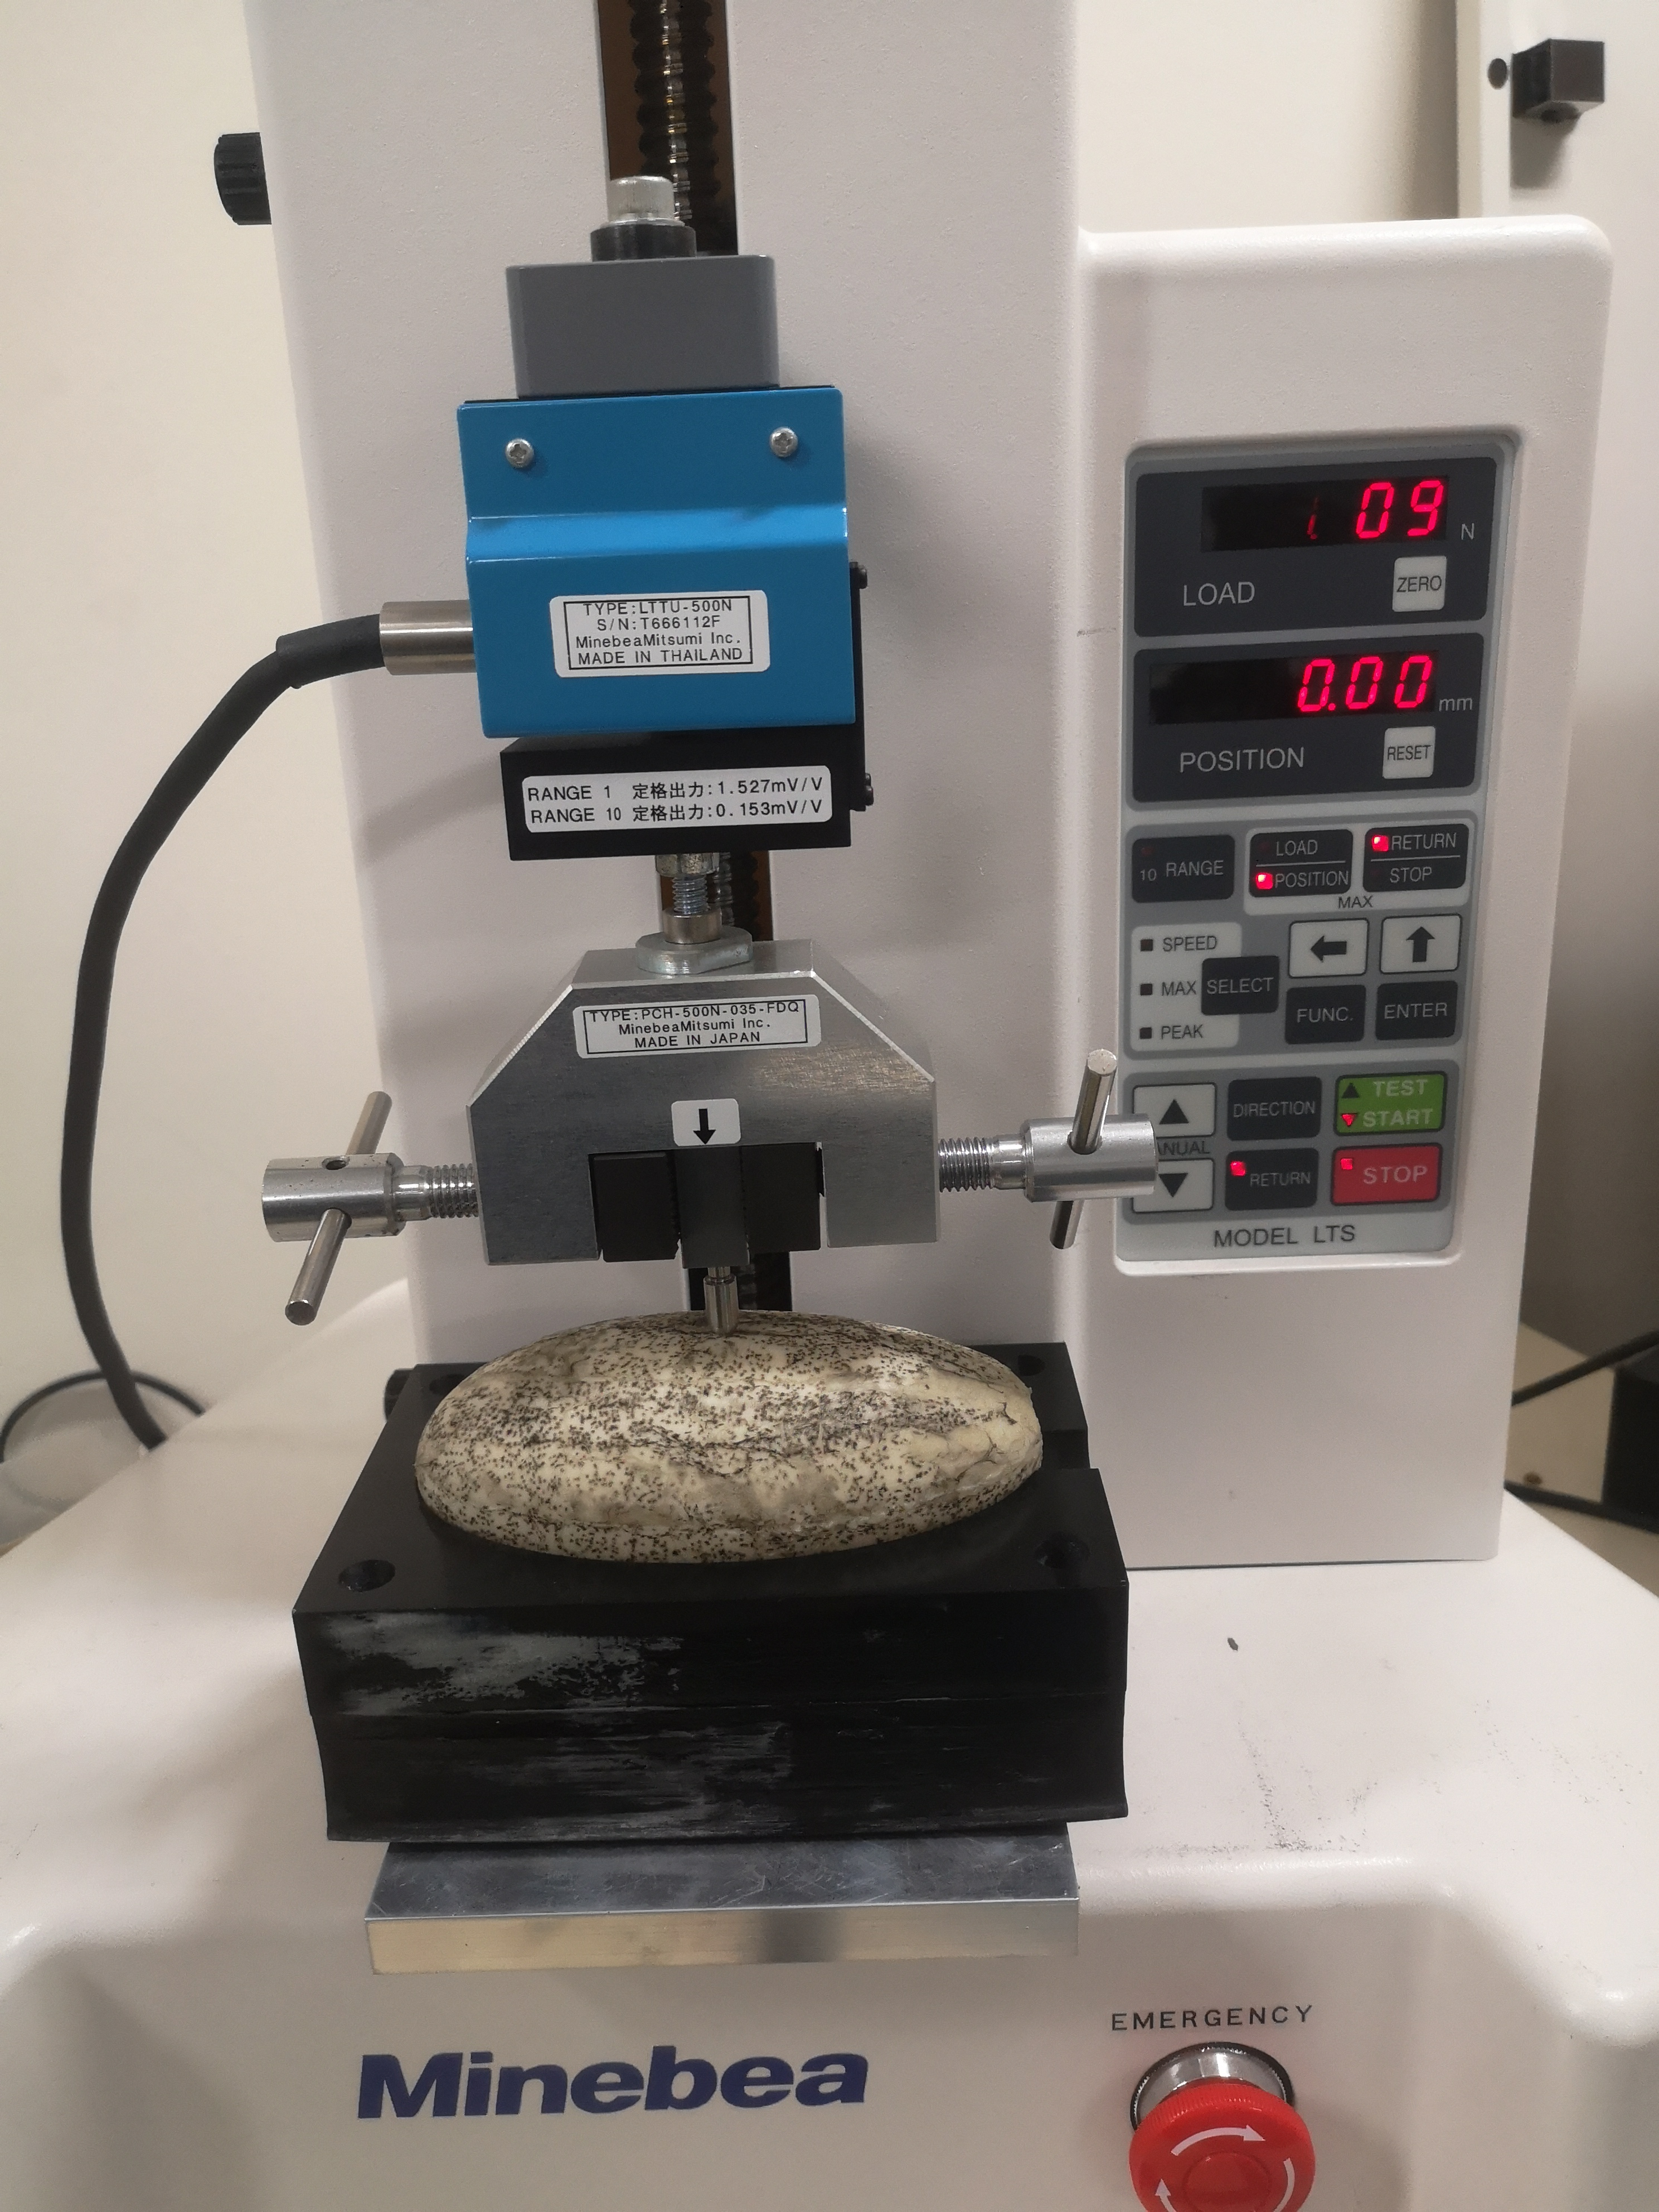
\includegraphics[width=6.5cm]{Images/Experiment/firstexperiment}}}%
    \qquad
    \subfloat[\centering Indentation test configuration with a \SI{10}{\newton} load cell \label{fig:10loadcell}]{{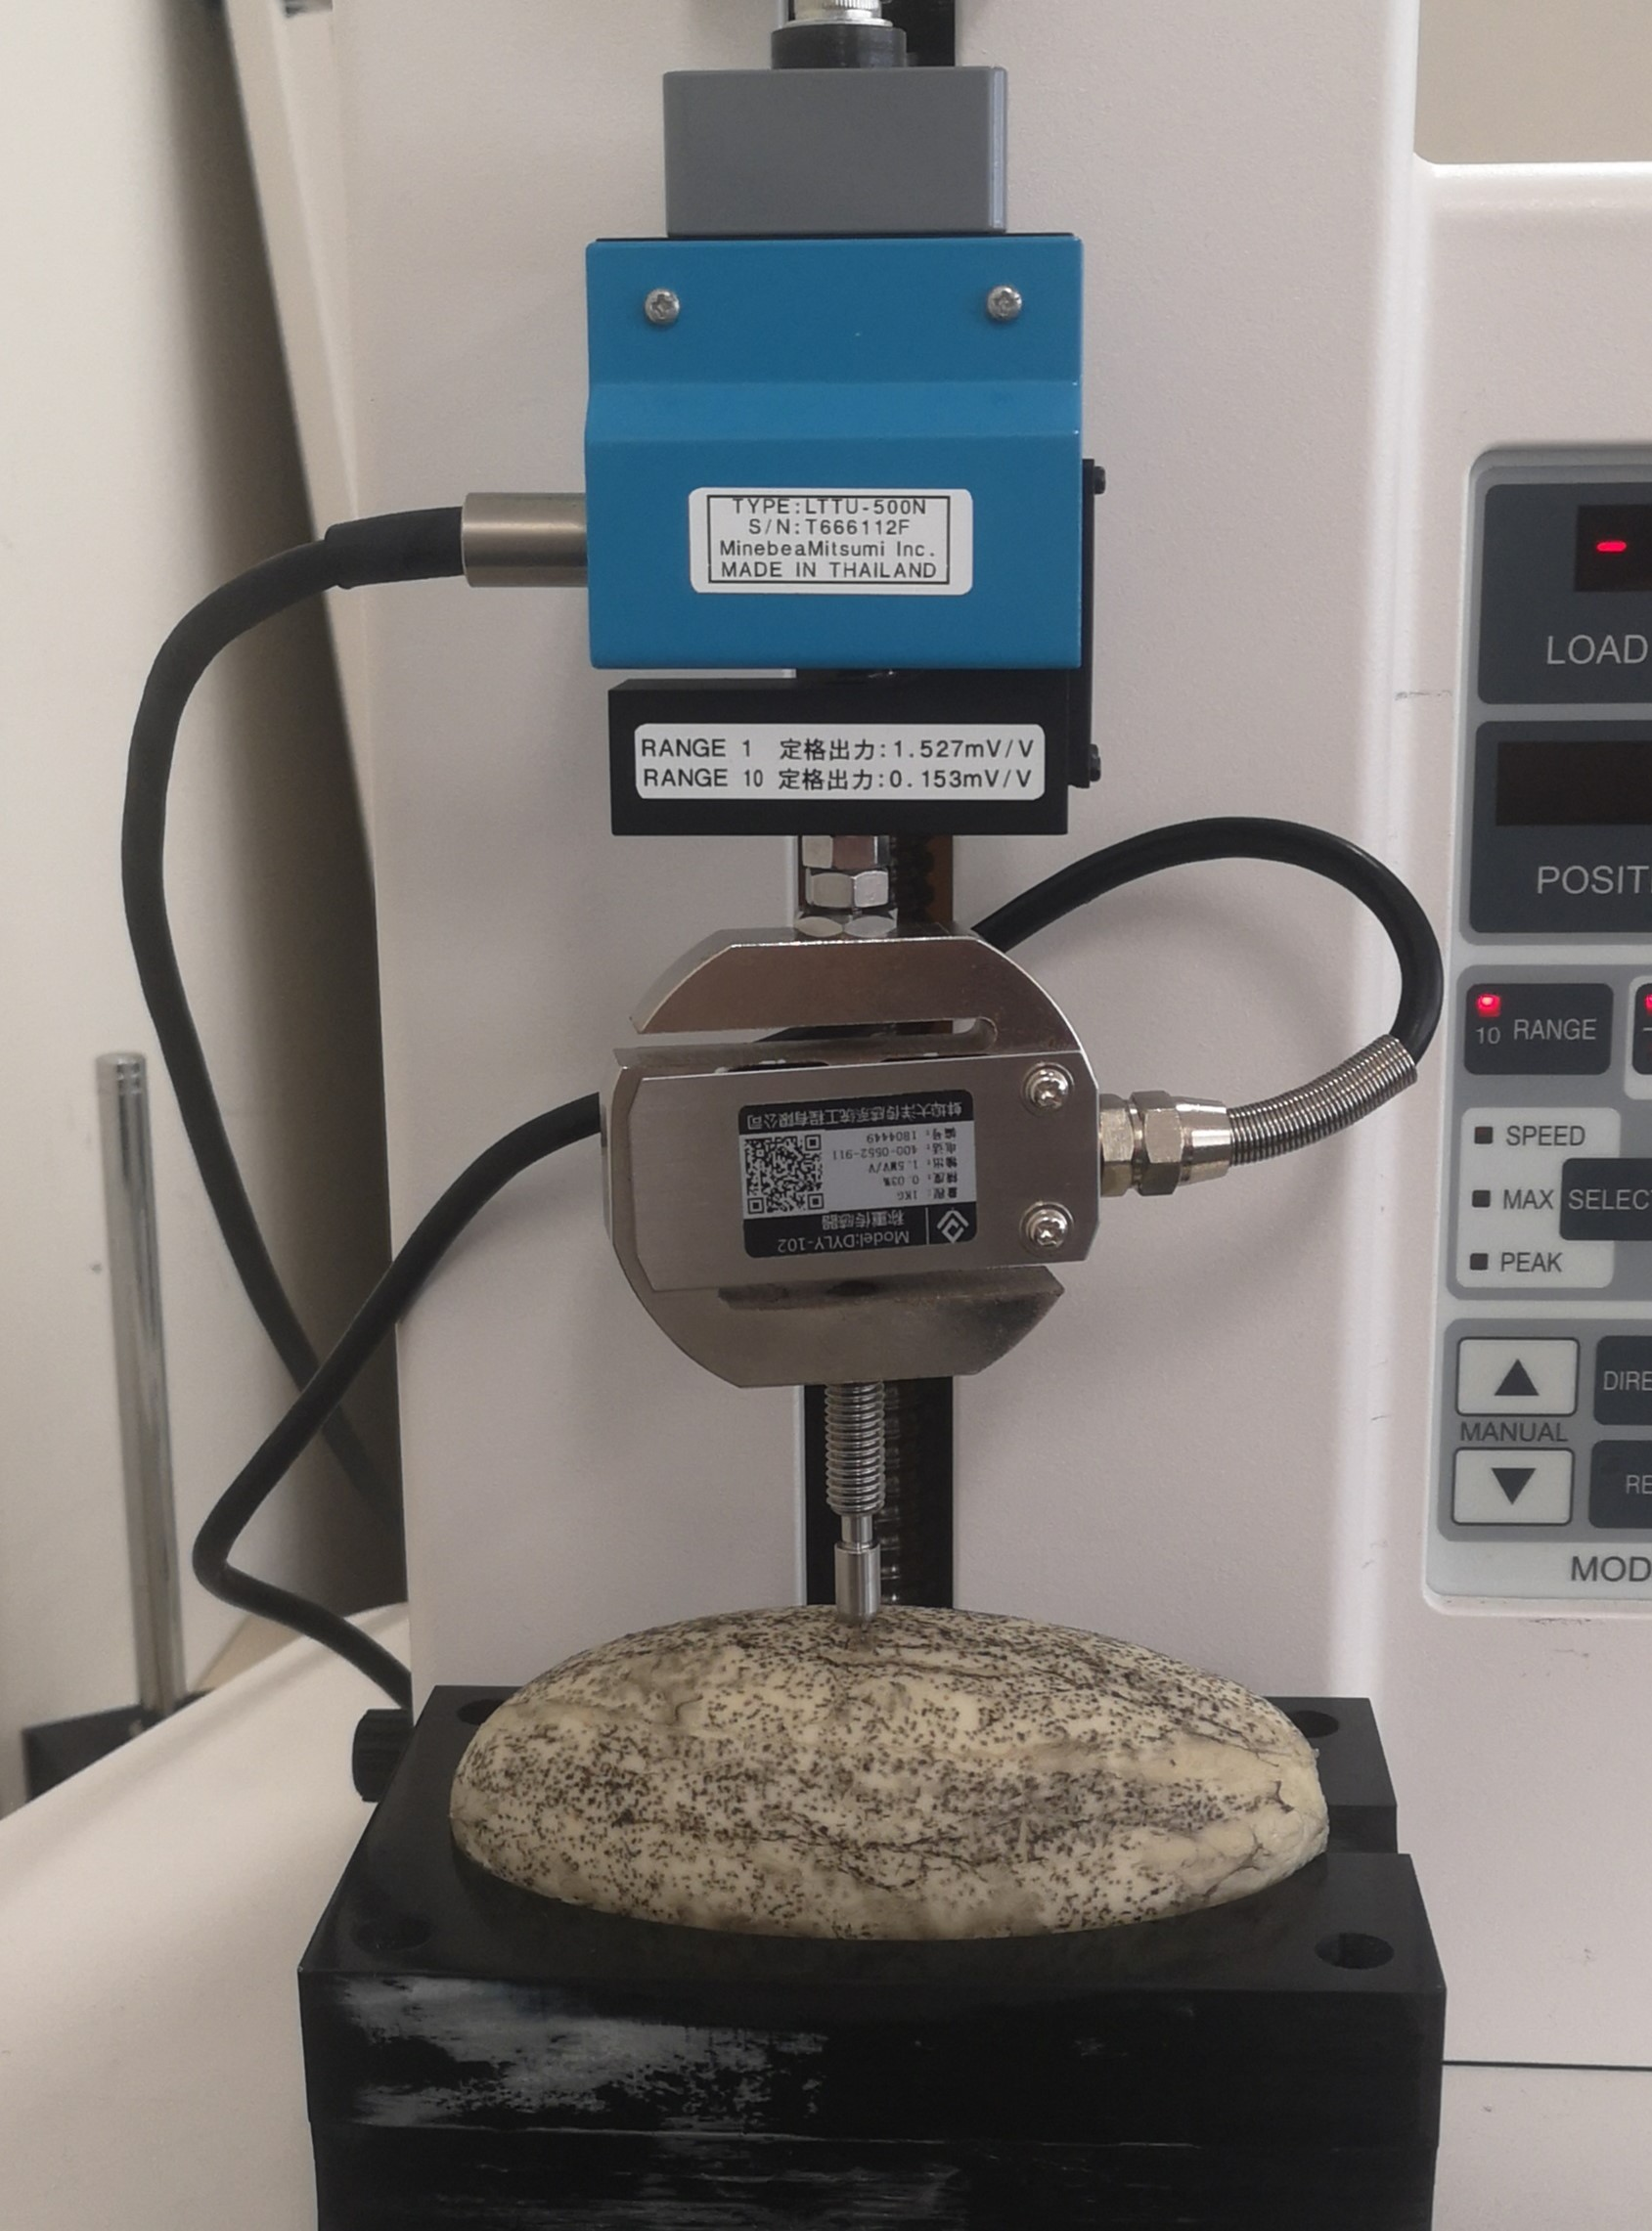
\includegraphics[width=6.5cm]{Images/Experiment/firstexpotherload}}}%
    \caption{First experimental model: Tensile and compression machine with an indenter with a rounded head. Test Specimen made from ultra-soft polyurethane resin positioned on a fixed platform with a similar shape for constraint.}%
    \label{fig:firstexperiment}%
\end{figure}


The test specimen used for this experiment was a ultra-soft polyurethane resin. 
As shown in Fig.. the specimen possesses a ellipsoidal form with 
with a minor radius \(r_1\) = 35 mm and a major radius \(r_2\) = 60 mm. This was positioned
 on a fixed platform that suited the ellipsoidal geometry of the 
 specimen to constrain its movement. 
 The specimen was tested in a indentation test configuration with a tensile/compression machine.
 To achieve this congiguration a pin with a rounded head made of structural steel, 
 with a radius of \(r_3\) = 3 mm was attached 
 to the holding grips followed by a force load cell. 
The result of indentation test was a load-displacement points. The approximated 
polynomial curve was used as a reference for the material modeling.

%test specimen is loaded at a quasi-static rate

 The measured force reation \(F_1\) data showed a very small number, so the 
 first 50 N load cell displayed a lot of noise in the measurements. 
 Therefore, the load cell was change to 10N to reduce this interference. 
The 10 N load cell displayed the force-displacement curve of the indenter and the specimen
 in a finer way. Furthermore, in order to get the measurement of the load and 
 unloading process of
 the indentation a displacement sensor was attached to the tensile machine.

 The indentation depth \(h_1\) selected for the first model was 3,8 mm on the middle of the 
 top surface of the specimen. This indentation depth surpasses the pin radius \(r_3\) and 
 was chose arbitriarily to analyze the behavior of the material on the defined position.
 %reference?
 Additionally, it was observed that in soft materials it is easier to capture 
 some parameters with a larger indentation. Some references also observe that with
 indentation depth lower than indenter radius has a lot of noise and do not describe
 th results accurately. %reference?

 %results
 From the first experimental model we can observe that the material shows a nonlinear 
 behavior and the maximum total force reaction \(F_1\) lies around 0.45 N. %poner el grafico
 Furthermore, when applying different speeds, as show in Fig. %add figure 
 it is also possible to observe that 
 the hysteresis increases. %poner los speeds
This increasement shows that the material possesses a viscoelastic behavior, however
as this increasement is not significantly, it is possible to neglect viscoelasticity for 
the first stages of the project.

\begin{figure}[th]
    \centering
    \begin{tikzpicture}
        %\pgfplotsset{%legend outside the plot
        %every axis legend/.append style={ at={(1.05,0.95)}, anchor=north west,legend columns = 1}}
        \begin{axis}[
            %axis lines=middle,
            %x label style={at={(axis description cs:0.5,-0.1)},anchor=north},
            %y label style={at={(axis description cs:-0.1,.5)},rotate=90,anchor=south},
            xlabel={Displacement $u [mm]$},
            ylabel={Force reaction in Z-Axis $F_z [N]$},
            legend pos= north west]
            
            \addplot+[smooth, mark size = 1pt] table [y=$Force$, x=Def]{Table/data1.dat};
            %\addplot+[smooth] table [y=Force, x=$Def$]{Table/data2.dat};
            \legend{Experimental data}%,$l_2$}
        \end{axis}
    \end{tikzpicture}
    \caption[Expdata]{Experimental Load-displacement curve.}
    \label{fig:testgraph}
\end{figure}

\section{Experimental Model II}
\label{section:expmod2}
%i.	Description of the experimental setup
%ii.	Procedure for conducting the experiment
%iii.	Analysis of different platforms

The second experimental model was developed by Yokohama National University. Similar to 
the first experimental model the test specimen and the platform were it lies, has the 
same dimensions, minor radius $r_1 = \SI{35}{\milli \m}$ and a major radius \(r_2\) of 60 mm. The
test specimen is also made from the same material, ultra-soft polyurethane resin.

The indenter on the other hand, is a sphere made of ruby, the sphere radius is also 
equal to the radius of the pin \(r_s\) 3 mm and attached to it, is the force load cell.

A laser is used to measure the displacement which results in a load-displacement curve.
With this model it is possible to not only determine the toal force reaction, but also
it's components \(F_x\),  \(F_y\) and \(F_z\). Furthermore, with the laser it is also
possible to observe the deformation not only in one point but around the whole area. 
This allows as to analyze the deformation of the whole structure.

The indentation speed selcted was % ask for which speeed
and with an indentation depth of \(h_s\) is 4 mm. With this experiment, 4 key points on 
the sepcimen's surface were chosen: First, in the middle and three other points, one to right, 
one down, and one diagonal to middle, forming a square with a distance between points 
of \(d_s\) 20 mm. %add figure with points




Similar to the previous model, Fig. % add 
shows a nonlinear behavior with a maximum force reac

\section{Experimental Tests Description}

\subsection{Middle Point}
\subsection{Load Unloading}
\subsection{Nearby Point}


\section{Analysis and Comparison of Experimental Techniques}

\subsection{Overview of the Data and Results}

\subsection{Main Assumptions for Material Modeling}



%----------------------------------------------------------------------------------
\section{Material model framework assumptions}

The first point to be analyzed, which is used to build a material model is point No. 1,
in the middle of the surface. The advantages from this case, is the less influence of
external factors. For this case it is vaiable to assumed, that shear stresses can be 
neglected and offers a simple model to focus on the material definition.

For this project, there is a focus on the limitation of each material model, 
departing from an ideal scenario. From this point on the material will be build 
accordingly and for each model the influence of the material parameters is going
to be assessed.

\subsection{First Material model}

\subsubsection{Linear elasticity}


\subsubsection{Hyperelasticity}
The strain energy density function for the Neo-Hookean material model is given with
\begin{align*}
            \Psi = C_1 (I_1 - 3) \, ,
\end{align*}
where $C_1$ is a material constant and $I_!$ is the first invariant of the right Cauchy-Green tensor. 
Neo Hookean and Mooney Rivlin comparison

%Crear chart

%----------------------------------------------------------------------------------
\section{Computational model}
The quasi static nature of the indentation experiment allows the use of a static 
structural analysis.

For the creation of the computational model, the SOLID 187 elements were used. The mesh 
for the whole model is formed from quad tetrahedral elemennts. The platform and 
the specimen have an global element size of 5 mm. The indenter has an element size of
0.5 mm. In the area of the indentation, there is finer mesh with an element size of
1 mm and a radius of 8 mm. 

Their a two main factors which increases the complexity of the validation of the simulation
and those are, the contact nonlinearity, and the element distortion due to indentation
 experiment. These issues make the computational time expensive, as it requires to manual 
 solutions for the meshing in the area of importance, and small time steps. 
 For that, 
 the nonlinear adaptive meshing option in ANSYS Workbench was applied, which does a remeshing
 process if the a certain parameter is exceeded.%Revisar explanation of nonlinear adaprive meshing
Specially, for larger indentation cases, this option shows a more stable model with a 
good mesh convergence analysis.

A force-displacement curve, shown in Fig... is generated from the first assumption, 
for this case 
%Additionally due to these factors, the converge analysis   

For both cases 
%----------------------------------------------------------------------------------
\section{Material model}

In an ideal and first scenario, this material can be assumed as linear, isotropic, 
elastic and nearly imcompressible. For this case, there are two main variables, the Young's
Modulus \(E\), and the Poisson's ratio $\nu$.

%comentario sobre la influencia del bulk modulus y poissons ratio
From the parametric analysis, it is possible to see that the bulk 
modulus of this material does not possess a big impact in the FE 
simulation results. This conclusion combined with the results 
from the Poisson ratio in the first material model coincide with the 
statements from Bergström, where it is no vital to know these parameters 
to obtain accurate FE computational models, as these have limited
influence on the mechanical response. \cite{Bergström2015} %pag64Bergströom

%---------------------------------------------------------------------------------